\chapter{Umstrukturierung und Innovation}

Als erstes gilt es herauszufinden welcher Teil des Code, der zuständig für das prompting ist, wie verbessert werden kann.
Das Projekt von TBA benutzt zur Erstellung von BPMN Diagrammen die OpenAI API und verwendet hier die bereitgestellte 
Technologie der Assistants.

\section{Generelle Umstrukturierungen}

Während der Code gut für seinen (bisherigen) speziellen Anwendungsfall ist, können hier einige Verbesserungen gemacht werden.

\subsection{Objektorientierter Ansatz}

Das Zeil ist es, den Code einfach erweiterbar und wartbar zu machen.
Hierfür ist es wichtig, den code möglichst schnell an Änderungen der OpenAI Api anpassen zu können.
Um das zu erreichen wird ein Objektorientierter Ansatz gewählt.
Die objektorientierte Programmierung bietet für den Aufbau des Prompting-Codes viele Vorteile und macht die Entwicklung 
langfristig übersichtlicher und wartbarer. 
Wir erstellen eine abstrakte Klasse `ai.ts' welche die gesamte Logik des Prompting beinhält und eine Klasse `openai.ts' 
welche von der AI Klasse erbt.
Die OpenAi Klasse muss nun nur noch Methoden implementieren, welche konkret auf die aktuelle version der API angepasst sind.
Durch die Verwendung von abstrakten Methoden wie generateContent(), createTitle() oder processResponse() wird sichergestellt, 
dass jede konkrete Implementierung dieselbe Schnittstelle einhält, 
aber ihre eigenen internen Abläufe definieren kann. 
Dies erleichtert den Austausch und die Erweiterung von Modellen, ohne den restlichen Code verändern zu müssen. 
Darüber hinaus werden wiederkehrende Prozesse, etwa das Speichern von Verläufen, das Verarbeiten von Antworten 
oder die Konvertierung zwischen Formaten, zentral in der Basisklasse gekapselt. 
Falls sich die API ändert, kann dies nun einfach in der Erbenden Klasse angepasst werden, ohne die dahinterliegenden Logik verändern zu müssen.

So sieht nun in abgespeckter Variante die Klasse für die OpenAI API aus.
Es gibt eine Methode \mintinline{typescript}{mapPromptInput();} um den Prompt in das richtige Format der API zu bringen,
\mintinline{typescript}{generateContent();} um den eigentlichen API aufruf durchzuführen und \mintinline{typescript}{preocessResponse();}
um die Antwort der API auszulesen.\\

\begin{samepage}
\begin{minted}[frame=single, framesep=2pt, linenos, fontsize=\small, style=vs]{typescript}
export class ChatGPT extends Ai {
  openai = new OpenAI({
    apiKey: OPENAI_API_KEY,
  });
  assist = await openai.beta.assistants.retrieve("asst_...");

  protected mapPromptInput(input) {
    return {
      input: input.prompt,
      model: this.model,
    };
  }

  protected async generateContent(input) {
    return await openai.beta.threads.runs.createAndPoll(
      thread_id, 
      { assistant_id: assist.id },
      { role: "user", content: input }
    );
  }

  protected processResponse(response) {
    return response.output_text.toString();
  }
}
\end{minted}
\end{samepage}

\subsection{Von Assistants zu Responses}

Die Änderungen welche im vorherigen Kapitel beschrieben wurden, zeigen gleich ihren Effekt, da OpenAI ankündigt ihre 
Assistants API einstellen zu wollen.
Sie emfehlen einen Umzug zu ihrer neuen Responses API.
Dies ist nun recht einfach umzusetzten, da wir nur die elementaren Methoden der API ändern müssen. 
So sieht nun die neue Methode \mintinline{typescript}{generateContent();} aus:\\

\begin{samepage}
\begin{minted}[frame=single, framesep=2pt, linenos, fontsize=\small, style=vs]{typescript}
protected async generateContent(input) {
  return this.openai.responses.create(input);
}
\end{minted}
\end{samepage}

Einer der zentralen Unterschiede zwischen der Assistants- und der Responses-API besteht darin, 
dass die System-Instructions bei der Verwendung der Responses-API manuell übergeben werden müssen. 
Dadurch ist es notwendig, die entsprechenden Anweisungen bei jeder Anfrage erneut mitzusenden. 
Dieser Umstand bringt jedoch nicht nur zusätzlichen Aufwand mit sich, sondern eröffnet auch neue Möglichkeiten: 
Die Instructions können flexibel und situationsabhängig angepasst werden, wodurch sich das Verhalten des Modells 
dynamisch steuern lässt.
Im folgenden Abschnitt wird gezeigt, wie dieser Ansatz weiter verbessert und effizienter gestaltet werden kann.

\subsection{Verbesserung der instructions}

Da die Instructions nun manuell mit jeder Anfrage übergeben werden, bietet sich die Möglichkeit, deren Aufbau 
gezielt zu optimieren. 
Ziel dieser Optimierung ist es, die Anzahl der benötigten Input-Tokens zu reduzieren, ohne dabei Qualität einzubüßen. 
Im besten Fall wird die Ausgabequalität sogar verbessert.
Der Assistant erhält als Grundlage zwei PDF-Dateien, die BPMN-Diagramme im Detail beschreiben, sowie zwei Textdateien: 
eine mit der Definition des verwendeten JSON-Formats und eine mit allgemeinen Regeln zum Aufbau der Diagramme. 
Die beiden PDF-Dokumente umfassen zusammen mehr als 10 MB und über 100 Seiten Text. 
Da ChatGPT bereits ein solides Grundverständnis von BPMN-Diagrammen besitzt, werden diese umfangreichen Dateien aus 
den Instructions entfernt. Mehrere Tests zeigen, dass sich diese Reduktion nicht negativ auf die Ergebnisqualität auswirkt. 
Dadurch lassen sich eine große Zahl an Tokens sowie Rechenzeit und Kosten einsparen.

Die beiden verbliebenen Textdokumente werden anschließend zusammengeführt, überarbeitet und in ein einheitliches, 
strukturiertes Format gebracht. 
Alle Regeln sind in einer geordneten Liste zusammengefasst und durch sogenanntes structured prompting klarer und 
maschinenlesbarer gestaltet. 
Ergänzend werden den Instructions zwei illustrative Beispiele hinzugefügt:
Zum einen ein minimales Beispiel, das den grundsätzlichen Aufbau des JSON-Formats verdeutlicht und die 
obligatorischen Elemente zeigt. 
Zum anderen ein umfangreicheres, praxisnahes Beispiel, das ein vollständiges BPMN-Diagramm mit allen relevanten Komponenten 
abbildet. 
Diese Kombination sorgt dafür, dass der Assistant sowohl einfache als auch komplexe Diagramme präzise interpretieren 
und reproduzieren kann.


\section{Formatauswahl}

Bisher wird die KI angewiesen, das Diagramm in einem eigens definierten JSON-Format zu erzeugen. 
Dieses Format wurde jedoch speziell für diesen Anwendungsfall entworfen und existiert in dieser Form nicht offiziell.
Entsprechend konnte das Modell während des Trainings kein Vorwissen darüber erwerben, sondern muss das Format 
ausschließlich auf Grundlage der bereitgestellten Instructions erlernen. 
Dadurch besteht die Möglichkeit, dass Fehler auftreten, etwa dann, wenn die Anweisungen unvollständig sind oder dem Modell 
bestimmte Kontextinformationen fehlen.

Um dieses Problem zu vermeiden, wird künftig die Option ergänzt, dass die KI ihre Ausgabe auch direkt im offiziellen 
Standardformat erzeugen kann. 
Das weltweit am häufigsten verwendete Austauschformat für BPMN-Diagramme ist XML, 
zu dem umfangreiche Dokumentation und etablierte Werkzeuge existieren. 
Dennoch bietet das eigens entwickelte JSON-Format einen entscheidenden Vorteil: 
Es besitzt eine deutlich höhere Informationsdichte und lässt sich dadurch kompakter und effizienter verarbeiten. 
Beide Formate haben somit ihre jeweiligen Stärken und Einsatzgebiete.

\begin{table}[H]
  \centering
  \renewcommand{\arraystretch}{1.2}
  \begin{tabular}{|p{2cm}|p{5.5cm}|p{5.5cm}|}
    \hline
    \textbf{Kriterium} & \textbf{JSON-Format} & \textbf{XML-Format} \\ \hline
    \textbf{Vorteile} &
    hohe Informationsdichte, geringer Tokenverbrauch, schnelle Generierung. &
    Standardisiert, gut dokumentiert, weit verbreitet, einfachere Instructions \\ \hline
    \textbf{Nachteile} &
    Kein Standard, Lernaufwand, komplizierter Konvertierungsalgorythmus. &
    hoher Tokenverbrauch, umfangreiche Syntax, unübersichtlicher, mehr Kosten, längere Generierung. \\ \hline
  \end{tabular}
  \caption{Vergleich der Vor- und Nachteile der unterstützten Ausgabeformate}
\end{table}

Für die Weiterentwicklung ist ein flexibles System das Ziel, das eine dynamische Auswahl des Ausgabeformats besitzt. 
Dadurch kann der Nutzer selbst entscheiden, welches Format im jeweiligen Anwendungsfall die besseren Ergebnisse liefert. 
Da sich die Formatwahl ähnlich wie die Wahl des verwendeten Modells direkt auf die Qualität der Ergebnisse auswirkt, 
wird die Auswahlmöglichkeit direkt in die Modellkonfiguration integriert. 
So kann beispielsweise zwischen Varianten wie `gpt-4.1-mini (xml)' und `gpt-4.1-mini (json)' gewählt werden. 
Wird kein Format angegeben, erfolgt die Ausgabe standardmäßig im XML-Format.

Eine Anfrage sieht damit z.B. folgendermaßen aus:\\

\begin{samepage}
\begin{minted}[frame=single, framesep=2pt, linenos, fontsize=\small, style=vs]{json}
// POST /threads
{ 
  "inputString": "Bitte generiere mir ein BPMN Diagram, 
      welches den Ablauf in einem Restaurant zeigt", 
  "model": "gpt-5 (xml)",
}
\end{minted}
\end{samepage}

Bei einer Anfrage kann dann die jeweilige AI über eine Map 

\mintinline{typescript}{const availableGPTs: Map<string, Ai>} 

zugeordnet werden, welche die Anfrage bearbeitet.

// TODO: update neuerungen noch machen


\section{Dateien}

Um die Qualität des Promptings weiter zu verbessern, soll eine Funktionalität implementiert werden, 
die es ermöglicht, auch Dateien direkt an die KI zu übermitteln. 
Dabei steht im Vordergrund, dass das Verfahren sowohl im Frontend als auch im Backend möglichst 
unkompliziert umgesetzt werden kann. 
Es soll keine aufwendigen oder zeitraubenden Konvertierungen erfordern und eine breite Auswahl an 
Dateitypen unterstützen, um die Nutzung so flexibel wie möglich zu gestalten.
Nach einer Analyse der OpenAI-Dokumentation unter
\url{https://platform.openai.com/docs/guides/images-vision?api-mode=responses&format=base64-encoded#analyze-images}
zeigt sich, dass die einfachste und zugleich effizienteste Methode zur Dateiübertragung die 
Verwendung einer Base64 Data URL ist. 
Diese Variante bietet eine einfache Möglichkeit, Binärdaten wie Bilder oder Dokumente direkt 
in Textform zu kodieren und zu übermitteln, ohne zusätzliche Infrastruktur oder spezielle 
Upload-Mechanismen zu benötigen.

Eine Base64 Data URL ist im eine Textdarstellung einer Datei, die direkt in eine URL eingebettet wird. 
Dabei werden die ursprünglichen Binärdaten in ein spezielles Textformat namens Base64 umgewandelt. 
Diese kodierten Daten beginnen typischerweise mit einer Kennzeichnung wie data:image/png;base64,\dots 
und enthalten danach die eigentlichen kodierten Inhalte. 
Der große Vorteil liegt darin, dass der Browser oder die API diesen Text automatisch wieder in die 
ursprüngliche Datei zurückwandeln kann. Auf diese Weise lassen sich Dateien direkt in 
JSON API-Anfragen integrieren, ohne dass zusätzliche Dateipfade, Server oder externe Speicherorte 
erforderlich sind. 
Dieses Verfahren ist daher besonders gut geeignet, um eine einfache, schnelle und universell 
kompatible Dateiübertragung zu ermöglichen.
Dadurch, dass die Datei nun einfach als String übergeben werden kann, können wir die Datei dem Body 
der Anfrage hinzufügen.

Eine Anfrage sieht damit z.B. folgendermaßen aus:\\

\begin{samepage}
\begin{minted}[frame=single, framesep=2pt, linenos, fontsize=\small, style=vs]{json}
// POST /threads
{ 
  "inputString": "Bitte generiere mir ein BPMN Diagram, 
      welches den Ablauf in einem Restaurant zeigt", 
  "model": "gpt-5 (xml)",
  "file": "data:image/png;base64,A35ekZ...",
}
\end{minted}
\end{samepage}

Der string wird auf Validität geprüft\\

\begin{samepage}
\begin{minted}[frame=single, framesep=2pt, linenos, fontsize=\small, style=vs]{typescript}
private checkBase64DataUrl(dataUrl: string): boolean {
  regex = /^data:([\w.+-]+\/[\w.+-]+)?;base64,[\w+\/]+=*$/;
  return regex.test(dataUrl);
}
\end{minted}
\end{samepage}

und dann im richtigen Format an die OpenAI API gesendet:\\

\begin{samepage}
\begin{minted}[frame=single, framesep=2pt, linenos, fontsize=\small, style=vs]{typescript}
const imageInstructions = {
  role: "user",
  content: [
    {
        type: "input_file",
        file_url: input.getFileDataUrl() as string,
    } as ResponseInputFile,
  ],
} as ResponseInputItem
\end{minted}
\end{samepage}

\section{Chain of Thought}

Um die Erzeugung und Interaktion rund um BPMN-Diagramme weiter zu verbessern, wird eine 
Technik implementiert, die als `Chain of Thought' bezeichnet wird. 
Dieses Verfahren ermöglicht es dem Modell, komplexere Denkprozesse intern nachzuvollziehen und 
schrittweise zu argumentieren, bevor eine Antwort erzeugt wird. 
Dadurch kann der Dialog natürlich und strukturiert verlaufen, da der Chatbot in der Lage ist, 
Zusammenhänge besser zu verstehen und über mehrere Gesprächsschritte hinweg Ergebnisse 
zu liefern.

Diese Erweiterung erlaubt es dem Nutzer, auf vielfältige Weise mit dem Chatbot zu interagieren: 
Es können Fragen gestellt, Ideen entwickelt, bestehende Diagramme erläutert oder 
Verbesserungsvorschläge erfragt werden. 
Der BPMN-Bot soll damit nicht nur ein Werkzeug für Diagrammerstellung bleiben, sondern sich zu einem 
vollwertigen, kontextbewussten Assistenten weiterentwickeln, der beim gesamten Modellierungsprozess 
unterstützt.

Darüber hinaus ist vorgesehen, dass der Chatbot selbstständig Rückfragen stellt, wenn bestimmte 
Angaben unvollständig, mehrdeutig oder widersprüchlich sind. 
So kann ein interaktiver Dialog entstehen, in dem beide Seiten aktiv zum Verständnis und zur Qualität 
der Diagrammerstellung beitragen. 
Um dies zu ermöglichen, benötigt der Chatbot Zugriff auf den bisherigen Gesprächsverlauf sowie auf 
den aktuellen Zustand des jeweiligen Diagramms. 
Nur durch diese Kontextkenntnis kann die KI präzise, nachvollziehbare und qualitativ hochwertige 
Antworten generieren.

\subsection{Implementierung eines neuen Modus}

Um die Erstellung von Diagrammen für den Nutzer nicht unnötig zu verkomplizieren,
bleibt die direkte Generierung eines BPMN-Diagramms weiterhin bestehen. 
Gleichzeitig soll jedoch mehr Flexibilität bei der Art der Interaktion geboten werden. 
Zu diesem Zweck wird der Anfrage ein zusätzlicher Parameter hinzugefügt, 
der das Antwortverhalten der KI steuert.

Über den Parameter \texttt{mode} kann festgelegt werden, in welchem Modus die
KI reagieren soll. 
Der bisherige Modus, bei dem ausschließlich das Diagramm
erzeugt wird, trägt nun die Bezeichnung \texttt{quick}. 
In diesem Modus erfolgt die Ausgabe direkt und ohne weiteren Dialog.

Der neu eingeführte Modus \texttt{detail} aktiviert den sogenannten
`Chain of Thought'-Ansatz. In diesem Modus verhält sich die KI dialogorientiert.
Sie kann Rückfragen stellen, Überlegungen anstellen oder alternative Vorschläge
anbieten, bevor das endgültige Diagramm erstellt wird. Dadurch entsteht eine
interaktive Konversation, die vor allem bei komplexeren Prozessen oder
unvollständigen Eingaben von Vorteil ist.

Eine Anfrage, die eine solche erweiterte Unterhaltung ermöglicht, könnte
beispielsweise folgendermaßen aussehen:\\

\begin{samepage}
\begin{minted}[frame=single, framesep=2pt, linenos, fontsize=\small, style=vs]{json}
// POST /threads
{ 
  "inputString": "Bitte schlag drei Prozessbeschreibungen 
    vor, aus denen dann eine ausgewählt wird um ein Diagramm
    zu erstellen.", 
  "model": "gpt-5 (xml)",
  "mode": "detail",
}
\end{minted}
\end{samepage}

\subsection{Konversationskontext}

Da es nun darum geht ein Chat zu implementieren, bei dem die KI möglichst gut auf Nachrichten reagieren
kann, ist es wichtig, dass die KI zugriff auf vorherige Nachrichten sowie auf das Diagramm hat.
Wäre das nicht der Fall, könnte die KI keine Fragen über das Diagramm beantworten und auch keine 
richtige Unterhaltung führen, da immer nur die aktuelle Nachricht bereitgestellt wird.
Bei LLM Anbietern wie OpenAI ist es notwendig, dass die Nachrichten historie in der Anfrage 
mitgeschickt wird.

Hierfür müssen alle Nachrichten eines Theads aus der Datenbank geladen werden.
Die Nachrichten werden dann auf wesentliche gefiltert und auf ein kompaktes Foramt gebracht.
Die OpenAI Klasse muss dann nur noch die Nachrichten auf das gefoderte Format bringen und in der
Anfrage mitschicken.
Da die Anfagen an die KI immer komplexer werden, wird nun eine Klasse $PromptInput$ angelegt.
Diese Klasse beinhaltet alle Informationen welche der KI mitgesendet werden sollen.
Bei einer erstellung diese Objekt können alle Rohdaten wie Instructions, Dateien oder der Chatverlauf
übergebe werden, welche die Klasse dann automatisch formatiert.
Ein entscheidender Schritt hierbei ist es die Teile der Nachrichten zu entfernen, in denen die KI mit einem
Diagramm geantwortet hat.
Das ist wichtig, da die Diagramme viele Tokens beinhalten und eigentlich nur das aktuellste Diagram 
wichtig ist. Hier bei kann es aber auch sein, dass das Diagramm noch vom Nutzer bearbeitet wurde.
Um dies zu berücksichtigen sind die Diagramme nuicht Teil der Nachrichten, welche mitgesendet werden.
Die Implementierung der KI-Schnittstelle kann anschließend ein Objekt der Klasse \texttt{PromptInput} 
entgegennehmen. 
Dieses Objekt dient als zentrale Datenstruktur, über die alle für die Anfrage relevanten Informationen 
an das Modell übergeben werden. 
Mithilfe vordefinierter Hilfsmethoden lässt sich der Inhalt komfortabel in das gewünschte 
Eingabeformat konvertieren, sodass keine manuelle Aufbereitung mehr erforderlich ist.

Die Klasse \texttt{PromptInput} verfügt über folgende Attribute:\\

\begin{samepage}
\begin{minted}[frame=single, framesep=2pt, linenos, fontsize=\small, style=vs]{typescript}
export class PromptInput {
  instructions: string[];
  history: {role: "user" | "assistant", content: string}[];
  prompt: string;
  file?: ;
}
\end{minted}
\end{samepage}

Damit ist es möglich, bestehende Nachrichtenverläufe aus der Datenbank abzurufen und automatisch in 
das benötigte Format zu überführen. 
Die Klasse übernimmt hierbei die vollständige Strukturierung der Daten, sodass diese
für die Kommunikation mit der KI genutzt werden können:\\

\begin{samepage}
\begin{minted}[frame=single, framesep=2pt, linenos, fontsize=\small, style=vs]{typescript}
const instructions = [formatInstructions, modeInstructions];
const chatsFromDB = getAllChatsFromDB(threadID);
new PromptInput(instructions, prompt, chatsFromDB, file);
\end{minted}
\end{samepage}

Das so erzeugte \texttt{PromptInput}-Objekt kann anschließend durch interne Methoden in das finale 
Format umgewandelt werden, das von der KI-Schnittstelle erwartet wird. 
Dadurch entsteht ein einheitlicher, wiederverwendbarer Datenfluss zwischen Anwendung, Datenbank und 
Modell, der die Wartung sowie zukünftige Erweiterungen vereinfacht.\\

\begin{samepage}
\begin{minted}[frame=single, framesep=2pt, linenos, fontsize=\small, style=vs]{typescript}
protected mapPromptInput(input: PromptInput) {   
  [...]
  const historyInstructions = input.history.map((item) => {
    return {role: item.role, content: item.content};
  });
  return {
    input: [systemInstructions, historyInstructions, 
            userInstructions, fileInstructions],
    model: this.model,
  };
}
\end{minted}
\end{samepage}

Darüber hinaus soll künftig auch die jeweils aktuellste Version des Diagramms an die Anfrage angehängt 
werden. 
Auf diese Weise erhält die KI den vollständigen Kontext und kann das bestehende Diagramm nicht nur 
bearbeiten, sondern auch inhaltliche Fragen dazu beantworten.

Da das aktuelle Diagramm nicht Bestandteil des eigentlichen Nachrichtenverlaufs ist, wird es in den 
sogenannten `System Instructions' hinterlegt. 
Diesen Instruction Block wird nun als `Update Instructions' bezeichnet und enthält stets die zuletzt 
gespeicherte Version des Diagramms. 
Die entsprechenden Daten werden automatisch aus der Datenbank geladen und vor dem Absenden der Anfrage 
in die System Instructions eingefügt.

Durch dieses Verfahren ist sichergestellt, dass die KI bei jeder Interaktion auf dem neuesten Stand 
bleibt und Änderungen im Diagramm jederzeit konsistent nachvollziehen kann.\\

\begin{samepage}
\begin{minted}[frame=single, framesep=2pt, linenos, fontsize=\small, style=vs]{typescript}
protected updateInstructions(threadID: string, format: format){
  const diagram = getLatestDiagramFromDB(threadID);
  return [`The The following diagram has already been created:
    ${format == "xml" ? diagram?.xml : diagram?.json}`]
}
\end{minted}
\end{samepage}

Damit hat die KI nun alle Informationen die sie benötigt um eine Konversation führen zu können.

\subsection{Konversationen} \label{konversationen}

Für eine vollständige Konversation benötigt die KI nun aber noch Anweisungen.
Dafür werden der KI noch die sogenannten $modeInstructions$ bereitgestellt.
Diese sehen zunächst so aus:\\

\begin{minted}[frame=single, framesep=2pt, linenos, fontsize=\small, style=vs]{text}
[Output Language depends on prompt language]

Alternative to creating a bpmn diagram you may ask any 
questions you feel like need answering to create the best bpmn 
diagram.
If you do not have any questions any more, please write a 
quick summary of the agreed diagram before creating the bpmn 
xml.
If the initial prompt is really basic provide the user with a 
creative scenario summary.

Once the user has agreed on a summary, Do no longer answer in 
plain text but only in bpmn xml.
If you want to provide questions, summary or any other type of 
text, that is not a diagram. Do not use JSON or XML. 
Only plain Text!
\end{minted}

Diese Instructions werden nur mitgesendet, falls der $detail$ modus genutzt wird.

Es ist nun eine Konversation möglich.

Wenn man den Bot nun fragt: ``Bitte schlag mir ein Diagramm vor'' antwortet dieser mit:

\setlist{nolistsep}
\noindent\fbox{
  \parbox{\textwidth}{
    Gerne, ich schlage Ihnen ein klassisches und leicht verständliches Szenario vor: 
    einen \textbf{Online-Bestellprozess}. 
    Dieses Diagramm würde die Interaktion zwischen einem Kunden und einem Online-Shop 
    darstellen und eignet sich gut, um grundlegende BPMN-Konzepte zu zeigen. 
    \textbf{Zusammenfassung des vorgeschlagenen Diagramms:} 
    \begin{itemize}[noitemsep]
      \item \textbf{Beteiligte (Pools):}
        \begin{enumerate}[noitemsep]
          \item Kunde
          \item Online-Shop
        \end{enumerate}
      \item \textbf{Ablauf beim Kunden:}
        \begin{enumerate}[noitemsep]
          \item Der Prozess beginnt damit, dass der Kunde ein Produkt auswählt.
          \item Er gibt eine Bestellung auf, was eine Nachricht an den Online-Shop sendet.
          \item Danach wartet er auf die Bestellbestätigung.
          \item Anschließend wartet er auf die Versandbestätigung.
          \item Der Prozess endet, wenn der Kunde die Ware erhalten hat.
        \end{enumerate}
      \item \textbf{Ablauf im Online-Shop:}
      \begin{enumerate}[noitemsep]
        \item Der Prozess startet, sobald die Bestellung des Kunden eingeht.
        \item Die Bestellung wird geprüft.
        \item Eine Entscheidung (Gateway): Ist der Artikel verfügbar?
          \begin{itemize}[noitemsep]
            \item \textbf{Ja:} Die Bestellung wird bestätigt (Nachricht an den Kunden), 
              die Ware wird verpackt und versendet. 
              Eine Versandbestätigung wird an den Kunden gesendet.
            \item \textbf{Nein:} Die Bestellung wird abgelehnt (Nachricht an den Kunden) 
              und der Prozess endet. 
          \end{itemize}
        \item Nach dem Versand der Ware ist der Prozess für den Shop abgeschlossen.
      \end{enumerate}
    \end{itemize}
    Dieses Szenario zeigt die Zusammenarbeit zwischen zwei Teilnehmern, den Austausch von 
    Nachrichten und eine einfache Geschäftsentscheidung. 
    Sind Sie mit diesem Vorschlag einverstanden? 
    Falls ja, erstelle ich das entsprechende BPMN 2.0 XML für Sie.
  }
}

Man kann darauf antworten mit ``Ja, bitte generier mir das Diagramm genau so wie beschrieben''.
Der Bot versteht, dass er nun nicht antworten, sondern ein Diagramm erstellen soll.
Daher sendet er nun kein Klartext sondern direkt ein BPMN XML.
Dieses sieht folgendermaßen aus:

\begin{figure}[ht]
  \centering
  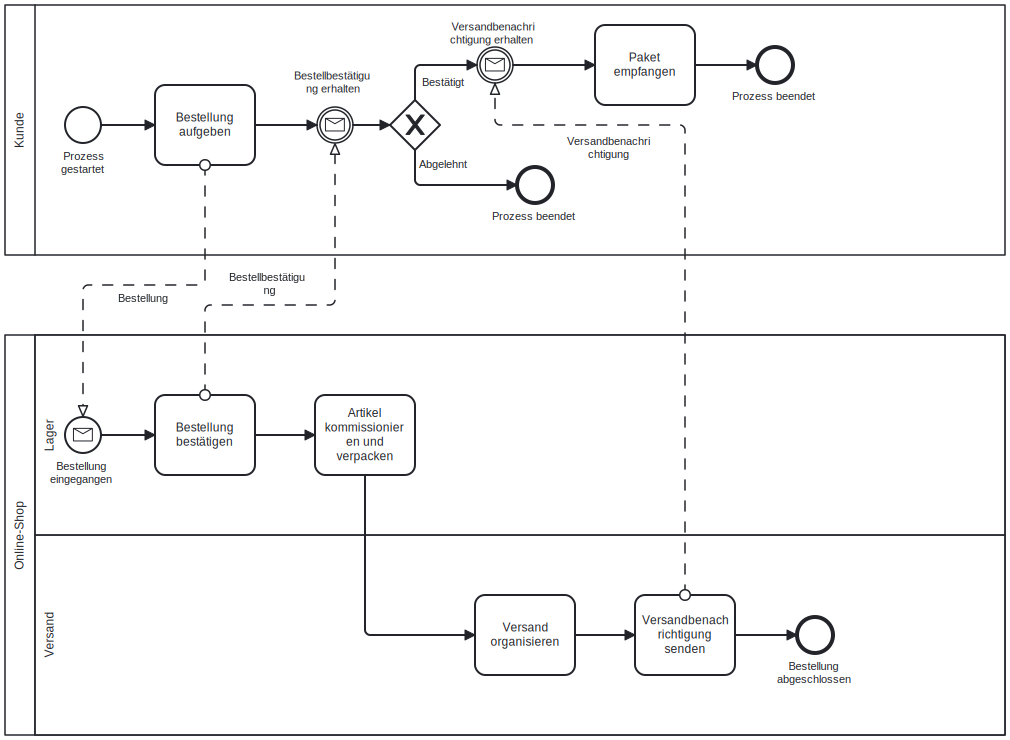
\includegraphics[width=\textwidth]{images/diagrams/diagram_1}
  \caption{\label{fig:diagram1}Beschreibung/Beschriftung des Bilds}
\end{figure}


Es fällt auf, dass der Bot das Gateway `Ist der Artikel verfügbar?' vergessen hat.
Dies ist allerdings kein Problem da das Diagramm nun weiter durch Prompts verbessern kann.
``Bitte bearbeite das Diagramm indem du das vergessene Gateway `Ist der Artikel verfügbar?' hinzufügst.''
Der Bot erkennt nun wieder, dass keine Textantwort gewünscht ist und beginnt mit der  
Übersendung des neuen Diagramms.

\begin{figure}[ht]
  \centering
  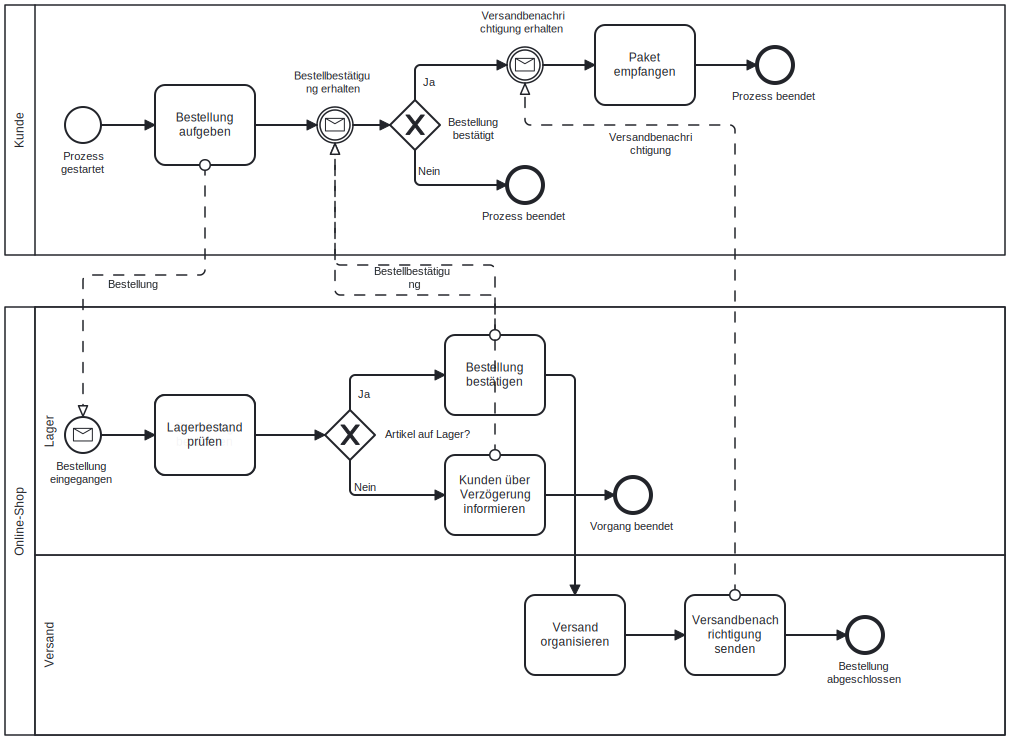
\includegraphics[width=\textwidth]{images/diagrams/diagram_2}
  \caption{\label{fig:diagram1}Beschreibung/Beschriftung des Bilds}
\end{figure}

Das Verhalten des ChatBots entspricht damit exakt den Anforderungen: 
Die Erstellung und Bearbeitung von Diagrammen kann vollständig interaktiv erfolgen, 
und der Nutzer erhält abhängig vom Kontext entweder Klartext oder direkt ein BPMN-Diagramm. 
Im gezeigten Beispiel war die Einordnung der Antwort relativ unkompliziert, 
da jeweils eindeutig erkennbar war, ob die KI ausschließlich Text oder ausschließlich ein 
Diagramm liefern sollte.

Für die weitere Entwicklung soll der Funktionsumfang jedoch erweitert werden, sodass der ChatBot 
künftig auch Antworten erzeugen kann, die Klartext und Diagramm gleichzeitig enthalten. 
Dadurch wird es möglich, dass der Bot zunächst eine Beschreibung, Analyse oder Erklärung liefert 
und anschließend unmittelbar ein dazugehöriges BPMN-Diagramm generiert. 
Ein solcher Anwendungsfall lässt sich beispielsweise mit einer Anfrage wie
„Zeig mir, was du so kannst, indem du eine Prozessbeschreibung erstellst und diese direkt in ein 
Diagramm umsetzt.“
simulieren.

In diesem Szenario entsteht eine neue Herausforderung: 
Die Antwort der KI besteht nicht mehr aus einer einzigen, klar abgrenzbaren Kategorie, 
sondern aus zwei unterschiedlichen Inhaltstypen, die voneinander getrennt verarbeitet werden 
müssen. 
Der Klartextteil soll wie gewohnt im Chat ausgegeben werden, während der Diagrammteil in das 
entsprechende Ausgabeformat überführt und anschließend angezeigt wird. 

Zu diesem Zweck wird ein zusätzlicher Erkennungsschritt eingeführt, der die Antwort der KI 
analysiert und die jeweiligen Segmente eindeutig identifiziert. 
Der ChatBot muss erkennen, welche Abschnitte in natürlicher Sprache formuliert sind und welche 
Bestandteile tatsächlich ein Diagramm darstellen, das weiterverarbeitet oder visualisiert werden 
soll. 
Dieses Verhalten ermöglicht eine deutlich flexiblere Interaktion und eröffnet neue 
Einsatzmöglichkeiten, besonders dann, wenn Nutzer sowohl inhaltliche Erläuterungen als auch die 
direkte Umsetzung in einem BPMN-Diagramm erwarten.

% evtl wieder entfernen:
Mit dieser Erweiterung entwickelt sich der BPMN-Bot zunehmend zu einem umfassenden 
Assistenzsystem, das nicht nur Modellierungsartefakte erzeugt, sondern auch begleitend erklärt, 
begründet und interaktiv mit dem Nutzer zusammenarbeitet.

Für dieses Kategorisierung wird eine Beispiel-Antwort betrachtet:

\noindent\fbox{
  \parbox{\textwidth}{
    Gerne, hier ist ein Vorschlag für einen einfachen, aber vollständigen Prozess: \\
    **Prozess:** Urlaubsantrag **Beteiligte:** Mitarbeiter, Vorgesetzter \\
    **Ablauf:** 1. Ein Mitarbeiter füllt einen Urlaubsantrag aus und reicht ihn ein. \\
    2. Der Vorgesetzte erhält den Antrag und prüft ihn. \\
    3. Der Vorgesetzte entscheidet, ob der Antrag genehmigt oder abgelehnt wird. \\
    * **Bei Genehmigung:** Der Mitarbeiter wird über die Genehmigung informiert. \\
    * **Bei Ablehnung:** Der Mitarbeiter wird über die Ablehnung informiert. \\
    4. Der Prozess ist in beiden Fällen abgeschlossen. \\
    \colorbox{black!0}{\strut\textasciigrave\textasciigrave\textasciigrave xml}%
    \colorbox{black!0}{\strut<?xml version=1.0 encoding=UTF-8?><bpmn:definitions}\\
    \colorbox{black!0}{\parbox{\linewidth-5pt}{\strut[\ldots]}}\\
    \colorbox{black!0}{\strut</bpmn:definitions>}%
    \colorbox{black!0}{\strut\textasciigrave\textasciigrave\textasciigrave}\\
    In diesem Beispiel gibt es ein \\ 
    \colorbox{black!0}{\strut<bpmn:startEvent name=``Urlaubsantrag ausgefüllt''>}
    , ein \\
    \colorbox{black!0}{\strut\textasciigrave}%
    \colorbox{black!0}{\strut<bpmn:exclusiveGateway name=``Antrag genehmigt?''>}%
    \colorbox{black!0}{\strut\textasciigrave}
    und weitere tasks welche den Ablauf eines Urlaubsantrags zeigen.
  }
}

Der Algorithmus soll nun zunächst alle Diagramme finden.
Dies wird hier durch den Aufruf eines Regex ermöglicht.

\begin{samepage}
\begin{minted}[frame=single, framesep=2pt, linenos, fontsize=\small, style=vs, breaklines, breakanywhere]{typescript}
/(?:``?`?\s*(?:xml)?\s*)?(<[^<>]*\/[^<>]*>\s*|<[^\/<>]*>[^`]*<\/[^<>]*>)+\s*(?:``?`?|(?=[^<>`\s]))\n?/g
\end{minted}
\end{samepage}

Über dieses werden automatisch alle validen XML Teile (In TBA label bunt markiert) erkannt.
Durch die Benutzung einer Non-capturing group werden Wrapper des XML 
(In TBA label blau markiert) wie zum Beispiel das 
`\textasciigrave\textasciigrave\textasciigrave xml', automatisch entfernt.
Alle matches werden danach auf ihre Länge geprüft um herauszufinden ob diese ein 
vollständiges Diagramm repräsentieren oder nur eine Referenz bzw. Erklärung als 
Teil des Klartextes sind. (In TBA label rot markiert)

\noindent\fbox{
  \parbox{\textwidth}{
    Gerne, hier ist ein Vorschlag für einen einfachen, aber vollständigen Prozess: \\
    **Prozess:** Urlaubsantrag **Beteiligte:** Mitarbeiter, Vorgesetzter \\
    **Ablauf:** 1. Ein Mitarbeiter füllt einen Urlaubsantrag aus und reicht ihn ein. \\
    2. Der Vorgesetzte erhält den Antrag und prüft ihn. \\
    3. Der Vorgesetzte entscheidet, ob der Antrag genehmigt oder abgelehnt wird. \\
    * **Bei Genehmigung:** Der Mitarbeiter wird über die Genehmigung informiert. \\
    * **Bei Ablehnung:** Der Mitarbeiter wird über die Ablehnung informiert. \\
    4. Der Prozess ist in beiden Fällen abgeschlossen. \\
    \colorbox{blue!60}{\strut\textasciigrave\textasciigrave\textasciigrave xml}%
    \colorbox{green!60}{\parbox{\linewidth-46pt}{\strut<?xml version=1.0 encoding=UTF-8?><bpmn:definitions}}\\
    \colorbox{green!60}{\parbox{\linewidth-5pt}{\strut[\ldots]}}\\
    \colorbox{green!60}{\strut</bpmn:definitions>}%
    \colorbox{blue!60}{\strut\textasciigrave\textasciigrave\textasciigrave}
    In diesem Beispiel gibt es ein \\ 
    \colorbox{red!60}{\strut<bpmn:startEvent name=``Urlaubsantrag ausgefüllt''>}
    , ein \\
    \colorbox{blue!60}{\strut\textasciigrave}%
    \colorbox{red!60}{\strut<bpmn:exclusiveGateway name=``Antrag genehmigt?''>}%
    \colorbox{blue!60}{\strut\textasciigrave}
    und weitere tasks welche den Ablauf eines Urlaubsantrags zeigen.
  }
}

Somit kann die gesamte Nachricht kategorisiert werden.
Grüne Teile sind Diagramme,
Nicht markierte Teile und rote Teile sind Teil der Klartextnachricht.

\section{Weitere Anbieter}

Es ist sinnvoll, dass der Chatbot neben ChatGPT auch andere Chatbot-Anbieter 
nutzen kann, um Flexibilität, Ausfallsicherheit und Vielfalt in den 
Antwortmöglichkeiten zu gewährleisten. 
Unterschiedliche Anbieter bieten verschiedene Stärken, wie etwa spezialisierte Natural 
Language Processing-Modelle, schnellere Antwortzeiten oder kosteneffizientere Lösungen. 
Durch die Integration mehrerer Anbieter kann der Bot je nach Bedarf die beste Leistung auswählen, 
alternative Perspektiven liefern und Ausfälle eines einzelnen Dienstes abfedern. 
Dies erhöht die Zuverlässigkeit und Qualität der generierten BPMN-Diagramme.

Durch die Objektorientierte Konfiguration der KI Schnittstelle ist es nun sehr einfach weitere 
Anbieter hinzuzufügen.
Im weiteren wird gezeigt wie weitere Anbieter nun hinzugefügt werden.

% TBA in den folgenden blöcken muss noch einiges getan werden. Kann man so nicht lassen.

\subsection{Grok}

% TBA umschreiben
Die Einbindung von Grok ergänzt ChatGPT, weil Grok schneller auf aktuelle Daten zugreift, oft 
direkter formuliert und technische Zusammenhänge sehr präzise erkennt. 
Dadurch kann der Bot bei bestimmten Aufgaben – etwa beim Interpretieren knapper Anweisungen 
oder beim Erzeugen alternativer BPMN-Varianten – Ergebnisse liefern, die ChatGPT allein nicht 
immer erreicht. 
Grok erhöht damit die Vielfalt, Genauigkeit und Zuverlässigkeit des Systems.

Grok kann einfach über die XAI SDK hinzugefügt werden.
Die Dokumentation findet man hier: \url{https://ai-sdk.dev/providers/ai-sdk-providers/xai}

Die zu versendende Nachricht an die Grok API muss nun nur noch vom PromptInput Objekt auf das 
API Format gebracht werden.\\

\begin{samepage}
\begin{minted}[frame=single, framesep=2pt, linenos, fontsize=\small, style=vs]{typescript}
protected mapPromptInput(input: PromptInput) {
  const historyInst = input.history.map((item) => {
    return {role: item.role, content: item.content} ;
  })
  const fileInst = input.file ? {
    role: "user",
    content: [{
      type: "image",
      image: input.getFileDataUrl() ,
    }],
  } : [];
  const userInst = {role: "user", content: input.prompt}
  return {
    model: this.xai(this.model),
    system: input.instructions.join("\n"),
    messages: [historyInst, userInst, fileInst],
  };
}
\end{minted}
\end{samepage}


\subsection{Gemini}

Die Einbindung von Gemini ergänzt ChatGPT, weil Gemini bei komplexen Analyseaufgaben, 
strukturiertem Denken und dem Umgang mit großen Informationsmengen besonders stark ist. 
Dadurch kann der Bot bei der Modellierung und Optimierung von BPMN-Prozessen zusätzliche 
Präzision und alternative Lösungswege bieten. Gemini erhöht so die fachliche Tiefe, Robustheit 
und Variantenvielfalt der Ergebnisse.\\

\begin{samepage}
\begin{minted}[frame=single, framesep=2pt, linenos, fontsize=\small, style=vs]{typescript}
protected mapPromptInput(input: PromptInput) {
  const systemInst = input.instructions.map((instruction) => {
    return {
      role: "model", 
      parts: [{text: instruction, thought: false}]
    };
  });
  const historyInst = input.history.map((item) => {
    return {
      role: item.role == "user" ? "user" : "model",
      parts: [{
        text: item.content, 
        thought: item.role == "assistant"
      }],
    };
  });
  const imageInst = input.file ? {
    role: "user",
    parts: [{
      type: "input_file",
      inlineData: {
        data: input.getFileBase64Data(),
        mimeType: input.getFileMimeType(),
      },
    }],
    } : [];
  const userInst = {
    role: "user", 
    parts: [{text: input.prompt}]
  };
  return {
    model: this.model,
    contents: [systemInst, historyInst, userInst, imageInst],
  };
}
\end{minted}
\end{samepage}

Die Gemini API erwartet bei Jedem Text Teil der Anfrage noch das Feld `thought', welches angibt
ob dieser Teil bereit von einer KI gedacht wurde.\\

\subsection{Claude}

\begin{samepage}
\begin{minted}[frame=single, framesep=2pt, linenos, fontsize=\small, style=vs]{typescript}
protected mapPromptInput(input: PromptInput) {
  const systemInst = input.instructions.map((instruction) => {
    return {type: "text", text: instruction};
  });
  const historyInst = input.history.map((item) => {
    return {role: item.role, content: item.content};
  });
  const imageInst = input.file ? {
    role: "user",
    content: [{
      type: "file",
      source: {
        type: 'base64',
        data: input.getFileBase64Data(),
        media_type: input.getFileMimeType(),
      },
    }],
  } : [];
  const userInst = {role: "user", content: input.prompt};
  return {
      model: this.model,
      max_tokens: 15000,
      system: systemInst,
      messages: [historyInst, userInst, imageInst],
  };
}
\end{minted}
\end{samepage}

\section{Streaming}

Bisher ergab es nur begrenzt Sinn, die Antworten der KI zu streamen, da ein Diagramm erst dann 
nutzbar ist, wenn es vollständig erzeugt wurde. 
Einzelne, unvollständige Fragmente eines BPMN-Diagramms bieten keinen Mehrwert und können vom 
Client nicht sinnvoll verarbeitet oder angezeigt werden. 
Mit der Einführung gemischter Antworten, die sowohl Klartext als auch Diagramme enthalten können, 
ändert sich dies jedoch.

Sobald ein Teil der Antwort aus natürlicher Sprache besteht, entsteht ein klarer Vorteil beim 
Streaming. 
Textinhalte können bereits angezeigt werden, während der restliche Output noch generiert wird. 
Dadurch erhält der Nutzer deutlich schneller Rückmeldung, was insbesondere bei komplexeren oder 
längeren Antworten zu einem spürbar verbesserten Nutzungserlebnis führt.

Technisch bedeutet dies, dass die Ausgabe der KI zunächst an den BPMNGen-Server gestreamt werden 
muss, der die eingehenden Daten analysiert und korrekt kategorisiert. 
Anschließend wird der Klartext Teil der Antwort weiter an den Client gestreamt. 
Entscheidend ist dabei, dass ausschließlich der textuelle Anteil der Antwort übertragen wird. 
Diagrammfragmente oder Codeblöcke würden beim Client zu Fehlern führen, da diese erst nach 
vollständiger Generierung sinnvoll weiterverarbeitet oder angezeigt werden können.

Durch diese Trennung entsteht ein effizientes zweistufiges Streaming-Verfahren: 
Der BPMNGen-Server verarbeitet die gesamte Antwort, extrahiert den Klartext in Echtzeit und 
leitet ihn unmittelbar weiter, während das Diagramm erst nach seiner vollständigen Fertigstellung 
bereitgestellt wird. 

Die gestreamte Ausgabe eines LLM-Anbieters zu starten ist in den meisten Fällen unkompliziert. 
Viele Modelle bieten dafür einen expliziten Parameter an, der direkt in der Anfrage gesetzt 
werden kann. 
Sowohl ChatGPT als auch Claude unterstützen dieses Vorgehen nativ, sodass sich das gewünschte 
Verhalten bereits beim Abschicken des Requests konfigurieren lässt. 
Ein entsprechendes Beispiel sieht wie folgt aus:\\

\begin{samepage}
\begin{minted}[frame=single, framesep=2pt, linenos, fontsize=\small, style=vs]{typescript}
protected mapPromptInput(input: PromptInput, stream: boolean) {
  [...]
  return {
    model: this.model,
    stream: stream,
    system: systemInst,
    input: [historyInst, userInst, imageInst]
  };
}
\end{minted}
\end{samepage}

Andere Anbieter wie Gemini oder Grok verfolgen dagegen einen leicht unterschiedlichen Ansatz und 
stellen das Streaming über eine separate API-Funktion bereit. 
Je nach verwendetem Endpunkt wird entweder ein normaler Text generiert oder ein Stream 
zurückgegeben. 
Der Wechsel zwischen beiden Varianten lässt sich dadurch einfach implementieren:\\

\begin{samepage}
\begin{minted}[frame=single, framesep=2pt, linenos, fontsize=\small, style=vs]{typescript}
async generateContent(input: any, stream: boolean) {
  if (stream) return streamText(input)
  return generateText(input);
}
\end{minted}
\end{samepage}

Sobald die Antwort der KI eintrifft, wird zunächst überprüft, ob es sich tatsächlich um einen 
Stream handelt. 
Da JavaScript-basierte Streams typischerweise das Symbol \texttt{asyncIterator} implementieren, 
lässt sich dies zuverlässig über eine einfache Typprüfung feststellen:\\

\begin{samepage}
\begin{minted}[frame=single, framesep=2pt, linenos, fontsize=\small, style=vs]{typescript}
protected isStream(obj: any): boolean {
  return obj && typeof obj[Symbol.asyncIterator] === "function";
}
\end{minted}
\end{samepage}

Wird ein Stream erkannt, kann dieser anschließend mithilfe eines asynchronen Iterations-Loops 
ausgelesen werden. 
Die empfangenen Delta-Fragmente lassen sich so in Echtzeit weiterverarbeiten, um 
Klartext sofort an den Client zu streamen, bevor das vollständige Diagramm erzeugt wird.\\

\begin{samepage}
\begin{minted}[frame=single, framesep=2pt, linenos, fontsize=\small, style=vs]{typescript}
protected async processStream(stream: any){
  for await (const chunk of stream) {
    switch (chunk.type) {
      case "response.output_text.delta":
        // Text oder andere Änderungen
        processDelta(chunk.delta);
        break;

      case "response.completed":
        // Fertig gelesen
        return;

      case "response.error":
      case "response.failed":
        // Fehler
        error(chunk.response.error.message);
        return;

      default:
        break;
    }
  }
}
\end{minted}
\end{samepage}

Während der Stream verarbeitet wird, wird die Antwort der KI schrittweise in einem internen 
Buffer aufgebaut. 
Nach jeder Erweiterung des Buffers wird der Klartextanteil, wie in Abschnitt \ref{konversationen}
beschrieben, extrahiert und an den Client weitergeleitet. 
Auf diese Weise erhält der Nutzer bereits während der Generierung der vollständigen Antwort 
fortlaufend Informationen, ohne auf das Endergebnis warten zu müssen.

Erkennt das System jedoch, dass der Stream gerade einen Diagrammteil enthält, wird dieser 
zunächst zurückgehalten und nicht an den Client übertragen. 
Diagrammfragmente sind während der laufenden Generierung weder syntaktisch vollständig noch 
anzeigbar. 
Es macht daher keinen Sinn diese zu streamen.

Sobald das Diagramm allerdings vollständig empfangen wurde, kann es analysiert und eindeutig 
einer Kategorie zugeordnet werden. 
Dabei wird, wie in Abschnitt \ref{konversationen} beschrieben, entschieden, ob es sich um ein 
finales BPMN-Diagramm handelt, das angezeigt werden soll, oder ob der betreffende Abschnitt 
lediglich Bestandteil eines beschreibenden Klartextes ist und somit kein eigenständiges 
Diagramm ist. 
Dieses Vorgehen stellt sicher, dass sowohl Text- als auch Diagrammausgaben sauber voneinander 
getrennt und jeweils korrekt verarbeitet werden, ohne dass unvollständige oder fehlerhafte 
Diagrammfragmente beim Client ankommen.

\subsection{SSE}

Für die Übertragung der erzeugten Informationen an den Client wird die Technik der Server-Sent 
Events (SSE) eingesetzt. 
SSE ermöglicht es dem Server, Daten in Echtzeit an den Client zu senden, ohne dass dieser 
wiederholt aktiv Anfragen stellen muss. 
Jede gesendete Nachricht folgt dabei einem strukturierten Aufbau und besteht aus zwei 
wesentlichen Komponenten: einem \texttt{event}-Feld und einem \texttt{data}-Feld.

Der \texttt{event}-Teil enthält in der Regel ein einzelnes Wort, das den Typ oder die Bedeutung 
der übertragenen Daten beschreibt, zum Beispiel \texttt{delta}, \texttt{diagram}, \texttt{error} 
oder \texttt{end}. 
Dadurch kann der Client umgehend erkennen, wie der empfangene Inhalt weiterzuverarbeiten ist.

Der eigentliche Inhalt befindet sich im \texttt{data}-Teil. 
Hier werden die Daten hinterlegt, beispielsweise ein Textdelta oder ein fertig generiertes 
Diagramm.

Zusammengefügt und korrekt formatiert wird die gesamte SSE-Nachricht schließlich in folgender 
Form an den Client übermittelt:

\noindent\fbox{
  \parbox{\textwidth}{
    event: \textit{event-name}\\
    data: \textit{Erste Zeile der Daten}\\
    data: \textit{Weitere Zeile mit Daten}\\

    event: \textit{Nächstes Event}\\
    \ldots
  }
}

Im folgenden wird nun gezeigt welche Events für die Übertragung einer Antwort an den Client
implementiert wurden.

Der Stream beginnt mit einem \texttt{start} Event. In diesem wird dem Client die Thread-ID mitgeteilt
und indirekt erkenntlich gemacht, dass nun ein Stream gestartet wird.

Da manche KI Anbieter Modelle entwickelt haben, welche zunächst Websuchen durchführen oder interne 
Prozesse durchführen,
kann es sein, dass zwischen dem Start des Streams und dem ersten Delta einiges an Zeit vergeht.
Um zu verhindern, dass der Browser des Clients deshalb durch einen Timeout die Verbindung schliesst,
wird das \texttt{alive} Event implementiert.
Dieses wird jede Sekunde gesendet und beinhaltet als data jedeglich die aktuelle Uhrzeit.

Das erste eigentliche Daten Event ist nun das \texttt{delta} Event bis dem die tatsächlichen
Deltas des Klartextteils versendet werden. 
Die Deltas haben keine fixe größe und können je nach LLM Anbieter und Antwort variieren.

Jegliche Fehler werden dem Client als \texttt{error} Event mitgleteil, wobei die Error Nachricht
als Data mitgesendet wird. Nach einem \texttt{error} Event wird die Verbindung automatisch vom 
Server beendet.

Wenn der Server erkennt, dass gerade ein vollständiges Diagramm erzeugt wird, sendet er ein
\texttt{diagram-start} Event welches dem Client mitteilt welche modell verwendet wird.
Sobald das Diagramm fertig erstellt wurde, wird auch ein \texttt{diagram-end} Event gesendet,
welches dem Client mitteilt, dass das Diagramm fertig erzeugt wurde,
sowie ein \texttt{diagram} Event gesendet, welches das fertige und formatierte Diagramm enthält.

Sobald der Stream des LLMs fertig ist, wird noch ein \texttt{end} Event versendet, welches die
gesamte Antwort als JSON versendet, genau so, wie die Antwort gewesen wäre, falls nicht an
den Client gestreamt worden wäre. Dies ist da um mögliche Fehler bei der Übersendung des Streams
ausbessern zu können.

Final wird noch ein \texttt{save} Event versendet, welches dem Client mitteilt, dass die generierte
Antwort nun auch erfolgreich in der Datenbank abgespeichert wurde und nun für weitere Anfragen 
bereit steht.
Danach wird der Stream geschlossen und die Übertragung ist abgeschlossen.

\noindent\fbox{
  \parbox{\textwidth}{
    event: start\\
    data: faf8ad85-5546-4da2-98d9-8784844f1ea9\\

    event: delta\\
    data: Ich bin\\

    event: delta\\
    data: ChatGPT 4.1 mini\\

    event: diagram-start\\
    data: gpt-4.1-mini\\

    event: alive\\
    data: 01.01.2025 00:02\\

    event: diagram-end\\
    data: gpt-4.1-mini\\

    event: diagram\\
    data: <?xml version=\textbackslash``1.0\textbackslash'' encoding=\textbackslash``UTF-8\textbackslash''?>\\
    data: <bpmn:definitions \ldots\\
    data: </bpmn:definitions>\\

    event: end\\
    data: \{ \\
    data: ``text'': ``Ich bin ChatGPT 4.1 mini''\\
    data: ``xml'': ``<?xml version=\textbackslash``1.0\textbackslash'' encoding=\textbackslash``UTF-8\textbackslash''?>\ldots</bpmn:definitions>''\\
    data: \}\\
    
    event: save\\
    data: success\\
  }
}

\section{Schema-Constraining}

\section{Evtl. Sampling}

\section{Evtl. Reflective Prompting}



